%%
%% Copyright 2007, 2008, 2009 Elsevier Ltd
%%
%% This file is part of the 'Elsarticle Bundle'.
%% ---------------------------------------------
%%
%% It may be distributed under the conditions of the LaTeX Project Public
%% License, either version 1.2 of this license or (at your option) any
%% later version.  The latest version of this license is in
%%    http://www.latex-project.org/lppl.txt
%% and version 1.2 or later is part of all distributions of LaTeX
%% version 1999/12/01 or later.
%%
%% The list of all files belonging to the 'Elsarticle Bundle' is
%% given in the file `manifest.txt'.
%%

%% Template article for Elsevier's document class `elsarticle'
%% with numbered style bibliographic references
%% SP 2008/03/01
%%
%%
%%
%% $Id: elsarticle-template-num.tex 4 2009-10-24 08:22:58Z rishi $
%%
%%
\documentclass[preprint,12pt,3p]{elsarticle}
\usepackage{graphicx}
\graphicspath{ {img/} }
%\documentclass[final,3p,times]{elsarticle}
%% Use the option review to obtain double line spacing
%% \documentclass[preprint,review,12pt]{elsarticle}

%% Use the options 1p,twocolumn; 3p; 3p,twocolumn; 5p; or 5p,twocolumn
%% for a journal layout:
%% \documentclass[final,1p,times]{elsarticle}
%% \documentclass[final,1p,times,twocolumn]{elsarticle}
%% \documentclass[final,3p,times]{elsarticle}
%% \documentclass[final,3p,times,twocolumn]{elsarticle}
%% \documentclass[final,5p,times]{elsarticle}
%% \documentclass[final,5p,times,twocolumn]{elsarticle}

%% if you use PostScript figures in your article
%% use the graphics package for simple commands
%% \usepackage{graphics}
%% or use the graphicx package for more complicated commands
%% \usepackage{graphicx}
%% or use the epsfig package if you prefer to use the old commands
%% \usepackage{epsfig}

%% The amssymb package provides various useful mathematical symbols
\usepackage{amssymb}
\usepackage{graphicx}
\usepackage[utf8]{inputenc}
%% The amsthm package provides extended theorem environments
%% \usepackage{amsthm}

%% The lineno packages adds line numbers. Start line numbering with
%% \begin{linenumbers}, end it with \end{linenumbers}. Or switch it on
%% for the whole article with \linenumbers after \end{frontmatter}.
%% \usepackage{lineno}

%% natbib.sty is loaded by default. However, natbib options can be
%% provided with \biboptions{...} command. Following options are
%% valid:

%%   round  -  round parentheses are used (default)
%%   square -  square brackets are used   [option]
%%   curly  -  curly braces are used      {option}
%%   angle  -  angle brackets are used    <option>
%%   semicolon  -  multiple citations separated by semi-colon
%%   colon  - same as semicolon, an earlier confusion
%%   comma  -  separated by comma
%%   numbers-  selects numerical citations
%%   super  -  numerical citations as superscripts
%%   sort   -  sorts multiple citations according to order in ref. list
%%   sort&compress   -  like sort, but also compresses numerical citations
%%   compress - compresses without sorting
%%
%% \biboptions{comma,round}

% \biboptions{}
\usepackage[procnames]{listings}
\usepackage{color}


\begin{document}

\begin{frontmatter}

\title{Assignment 1: Mixnets}

\author{Santiago Aragón}
\address{s.e.aragonramirez@student.utwente.nl}

\author{Owais Ahmed}
\address{o.ahmed@student.utwente.nl}
\address{University of Twente}

%\begin{abstract}
%Text of abstract. Text of abstract. %Text of abstract. Text of abstract. %Text of abstract.
%\end{abstract}


\end{frontmatter}

%%
%% Start line numbering here if you want
%%
% \linenumbers

%% main text



\section*{Assignment 1}
\begin{flushleft}
\textbf{Part A:}
We developed an application mixnets.py [Appendix A] to send messages via the three mix nodes and the cache node that forwards the individual messages to the recipient.
\newline

\textbf{Part B:}
We sent a message to TIM from the send message method as shown below in mixnets.py application [Appendix A].
\begin{verbatim}send_message('TIM     ','s1750542  and  s1736574') \end{verbatim}

\textbf{Part C:}

\begin{figure}[h]
\caption{Frequency of messages received against time in the same second.}
\centering
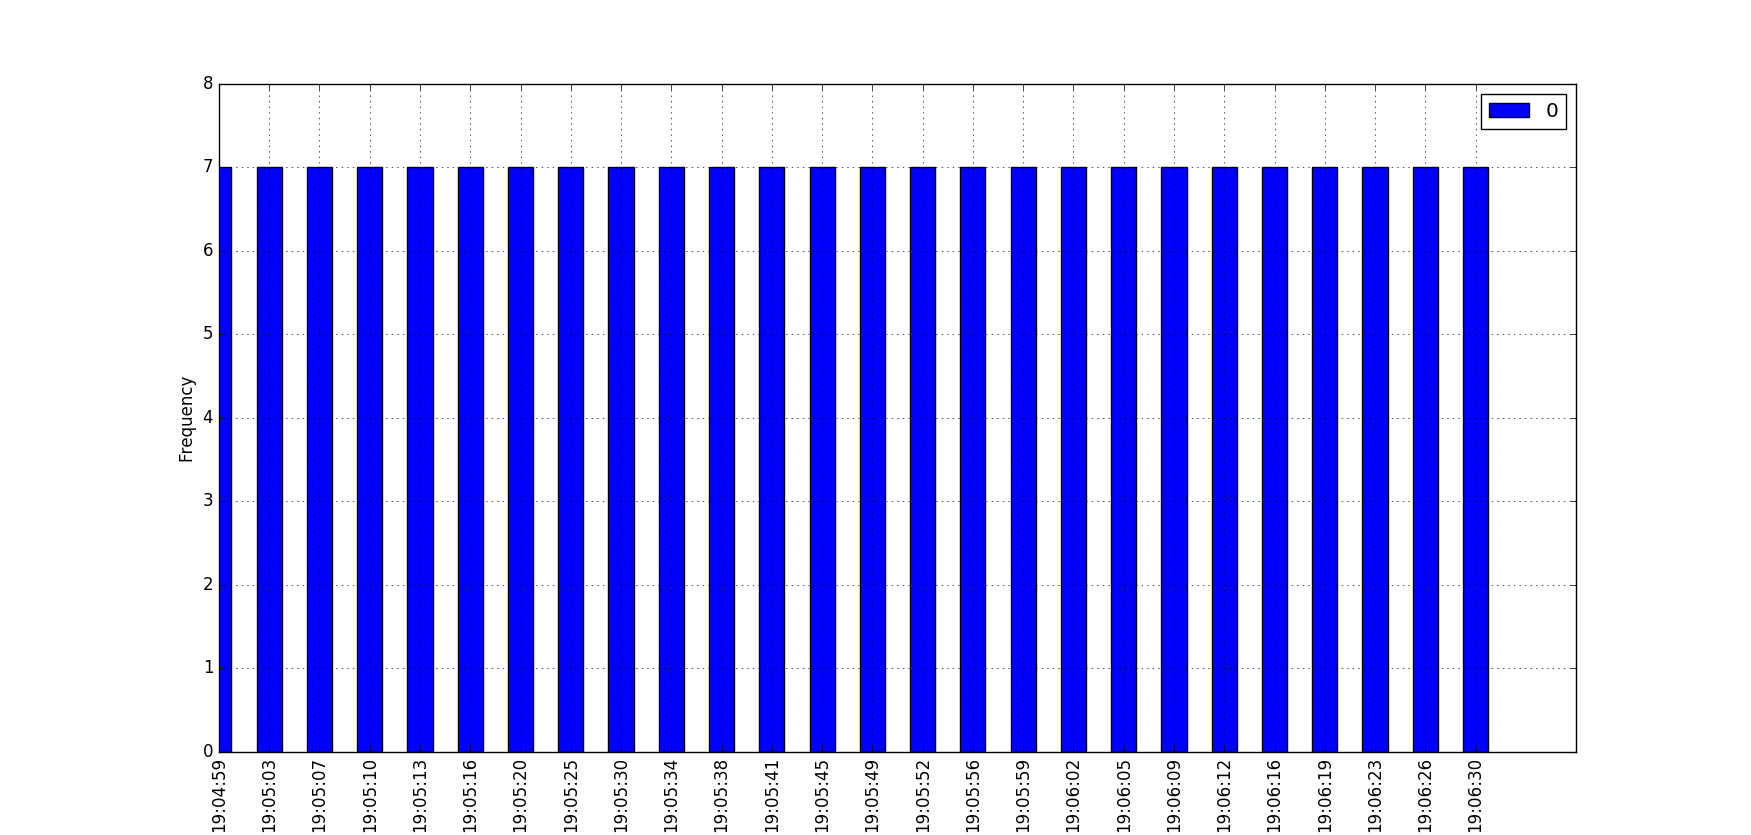
\includegraphics[width=\textwidth]{one_c}
\end{figure}

We parsed the cache log to analyse the individual messages and performed frequency analysis as shown in Figure: 1 by counting the number of messages received in a particular second and plotted the results in a bar chart graph. We observed that mostly seven messages were received in the cache log in a particular second, however in certain instances, the average of consecutive messages received in two seconds was seven. We therefore came to the conclusion that $n_C$ is 7, and since we know that the threshold of $n_A$ = $n_B$ = $n_C$, it implies that $n_A$ , $n_B$ and $n_C$ is 7.

\section*{Assignment 2}
\textbf{Part A:}
\newline

We sent individual messages one by one with a short time delay and observed the output via the cache log by parsing the message fields. We observed that the messages forwarded by MIX C to the CACHE NODE had a frequency of mostly 6 or 9. We learned that the sum of messages received in consecutive seconds was always a factor of 3, as shown in Figure: 2. We therefore, we came to the conclusion that the threshold of $n_C$ is 3.
\newline
\begin{figure}[h]
\caption{Frequency of messages received against time in the same second.}
\centering
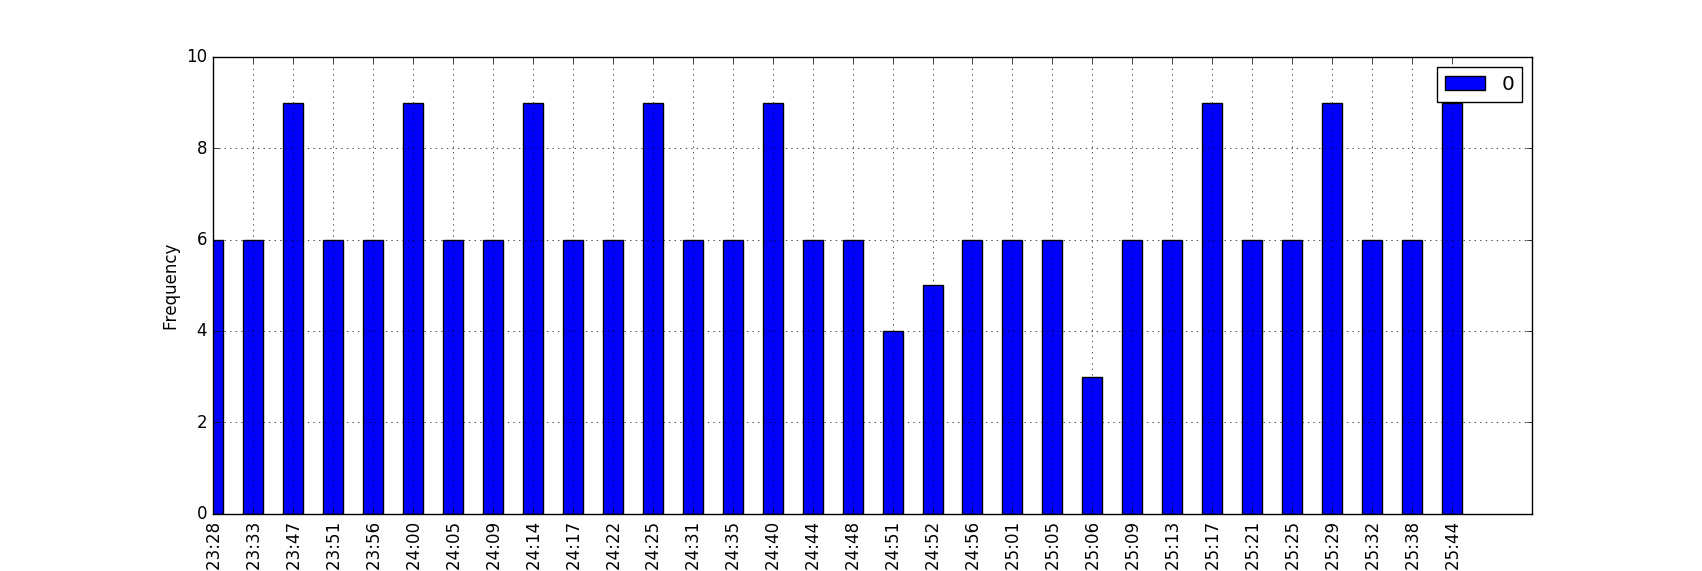
\includegraphics[width=\textwidth]{second}
\end{figure}
\newline
We kept a count of the messages entering the second mixnet via MIX A and the messages received in the cache log after reaching the threshold $n_C$. After the first 8 messages passed through MIX A, only 6 messages were displayed in the cache log. Since we know that the threshold of MIX B has to be at least more than $2n_C$ and less than $3n_C$. This implies that the threshold of MIX B is 6 $<$ $n_B$ $<$ 9. Furthermore, we have only inject 8 messages and we know that $n_A\geq 1$ , therefore we conclude that the threshold $n_B$ is 7.
\newline
\newline
We kept a count of the messages entering the second mixnet via MIX A and the messages received in the cache log after reaching the threshold $n_C$. After the first 8 messages passed through MIX A, only 6 messages were displayed in the cache log, that denotes that 1 $\leq$ $n_A, n_B$ $\leq$ 8. We sent more messages one by one until a second batch of 6 messages were received in the cache log. We noted that after sending 6 more messages, another batch of 6 messages was received in the cache log, this further helped us to analyse that MIX A always accepted even number of messages and the least common factor of the input messages to obtain an output was always 2. We therefore concluded that the threshold of $n_A$ is 2.

\begin{center}
Threshold of $n_A$ is 2

Threshold of $n_B$ is 7

Threshold of $n_C$ is 3
\end{center}




\textbf{Part B:}

\section*{Assignment 3}
\textbf{Part A:}

....
\newline


\textbf{Part B:}
....
\newline

\end{flushleft}

%% appendix sections are then done as normal sections
\appendix

\section{Mixnet 1}

\label{appendix-sec1}
%% References
%%
%% Following citation commands can be used in the body text:
%% Usage of \cite is as follows:
%%   \cite{key}         ==>>  [#]
%%   \cite[chap. 2]{key} ==>> [#, chap. 2]
%%
%% References with bibTeX database:

\bibliographystyle{elsarticle-num}
% \bibliographystyle{elsarticle-harv}
% \bibliographystyle{elsarticle-num-names}
% \bibliographystyle{model1a-num-names}
% \bibliographystyle{model1b-num-names}
% \bibliographystyle{model1c-num-names}
% \bibliographystyle{model1-num-names}
% \bibliographystyle{model2-names}
% \bibliographystyle{model3a-num-names}
% \bibliographystyle{model3-num-names}
% \bibliographystyle{model4-names}
% \bibliographystyle{model5-names}
% \bibliographystyle{model6-num-names}
\bibliography{sample}


\end{document}

%%
%% End of file `elsarticle-template-num.tex'.
